\chapter{Computertomographie}
\label{cha:1}

Der erste Teil dieses Kapitels gibt eine kurze Einführung in die Thematik der Computertomographie (CT). Es werden die Ideen und das Prinzip des CT-Vorgangs erklärt. Dies macht die Inhalte der späteren Kapitel besser verständlich. Eine detailreiche Einführung in die CT-Technik ist in \cite{Buzug04} aufgeführt.

Im zweiten Teil dieses Kapitels werden wir die Beobachtungen aus dem ersten Teil heranziehen und ein mathematisches Modell der Computertomographie aufstellen. Anschließend untersuchen wir einige Eigenschaften des aufgestellten Modells, die vor allem bei der Bildrekonstruktion aus tomographischen Daten eine wichtige Rolle spielen werden. 

\section{Das Prinzip des Computertomographen}
\label{cha:1.1}

Das Wort Tomographie setzt sich aus zwei dem Altgriechischen entstammten Wörtern zusammen. $\tau o\mu\eta$ [\textit{tome}], bedeutet Schnitt und $\gamma\rho\alpha\varphi\varepsilon\iota\nu$ [\textit{graphien}] bezeichnet Schreiben. Zusammengefasst zu einem Wort \textit{Tomographie} kann es als Schnittbild eines Objekts verstanden werden. 

Die CT ist ein bildgebendes Verfahren, das in der medizinischen Radiologie und in der Materialforschung eingesetzt wird. Die Technologie des Verfahrens erlaubt eine zerstörungsfreie Materialuntersuchung. Das ausschlaggebende Wort ist hier \textit{zerstörungsfrei}, damit ist die Untersuchung des inneren Aufbaus eines Objekts, ohne es zu öffnen, gemeint. 
%----------------------------------------------------------------------------------------
%	Beginn der Grafik
%----------------------------------------------------------------------------------------
\begin{figure}[!h]
	\centering
	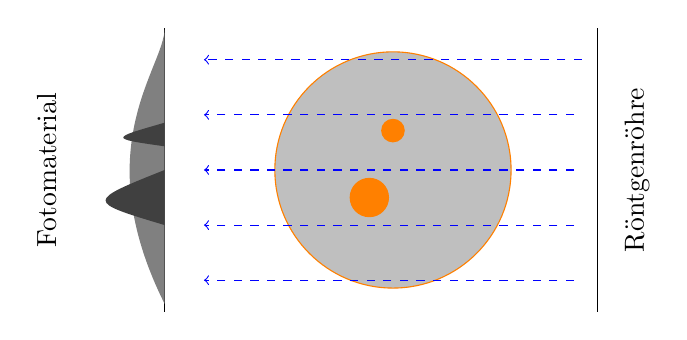
\begin{tikzpicture}[domain=3:3]  
	
	\fill[lightgray] (0.9,0.7) circle (1.5cm);
	
	\draw [rotate=90, yshift=2cm, -](-1.1,0) -- (2.5,0); % s-Achse
	
	\draw  (-0.5, 0.7) node [rotate=90, yshift=3cm] {Fotomaterial};
	
	\fill[gray] [rotate=90, yshift=2cm] (-1,0) .. controls (1,1) and (2,0) .. (2.5,0);
	\fill[darkgray] [rotate=90, yshift=2cm] (0,0) .. controls (0.3,1)  .. (0.7,0);
	\fill[darkgray] [rotate=90, yshift=2cm] (1,0) .. controls (1.1,0.7)  .. (1.3,0);
	
	\draw[orange] (0.9,0.7) circle (1.5cm);
	\fill[orange] (0.9,  1.2) circle (.15cm);
	\fill[orange] (0.6, 0.35) circle (.25cm);
	
	\draw [rotate=90, dashed, ->] [blue] (0,-3.2) -- (0,1.5); % strahl
	\draw [rotate=90, xshift=-0.7cm, dashed, ->] [blue] (0,-3.2) -- (0,1.5); % strahl
	\draw [rotate=90, xshift=0.7cm, dashed, ->] [blue] (0,-3.2) -- (0,1.5); % strahl
	\draw [rotate=90, xshift=1.4cm, dashed, ->] [blue] (0,-3.2) -- (0,1.5); % strahl
	\draw [rotate=90, xshift=2.1cm, dashed, ->] [blue] (0,-3.3) -- (0,1.5); % strahl
	
	\draw [rotate=90, yshift=-3.5cm, -](-1.1,0) -- (2.5,0); % Sensor-Achse
	\draw  (3, 0.7) node [rotate=90, yshift=-1cm, -] {Röntgenröhre};
	
	\begin{scope}[xshift=1cm]
	\end{scope}
	
	\end{tikzpicture}
	\caption{Schematischer Aufbau einer Röntgenaufnahme im Draufsicht. Links ist das Schwächungsprofil nach Durchgang der Röntgenstrahlen durch ein Medium mit verschiedenen Dichten zu sehen (mit der Annahme, dass orangene Kreise höhere Dichte haben, als die graue Fläche).}
	\label{fig:1.1}
\end{figure}
%----------------------------------------------------------------------------------------
%	Ende der Grafik
%----------------------------------------------------------------------------------------

Sicherlich wäre die Computertomographie ohne die Röntgenstrahlung nicht denkbar. Diese verdankt ihren Namen dem deutschen Physiker Wilhelm Conrad Röntgen (1845-1923). Im Jahre 1895 gelang es ihm zum ersten Mal eine elektromagnetische Strahlung zu erzeugen, deren Wellenlänge zwischen 10$nm$ und 1$pm$ lag. Solche kurze Wellenlängen haben nur energiereiche Strahlen. Das erlaubt ihnen die Durchdringung der Materie. Anzumerken ist, dass die Intensität hochenergetischer Strahlen beim Durchgehen der Materie mit der Eindringtiefe abfällt. Dies bedeutet, dass die Röntgenstrahlung beim Auftreffen auf ein Probestück eine höhere Intensität besitzt als beim Austreten. Bei den herkömmlichen Röntgenaufnahmen wurde diese Eigenschaft direkt ausgenutzt und man hat überlagerte Schatten von Objekten mit verschiedenen Dichten auf das Aufnahmematerial projiziert bekommen. Damit erschienen die dichteren Stellen des Objekts dunkler, weiche entsprechend heller. Für gewisse Situationen geben solche Projektionen genug Information her, jedoch nicht, wenn die räumliche Anordnung des Inneren eines Objekts diskutiert werden soll (Abb.\ref{fig:1.1}).

Um das Problem der räumlichen Anordnung der Objekte zu lösen, ist folgendes Vorgehen sehr nützlich. Würde man das Schattenbild aus der Abbildung \ref{fig:1.1} zurück in die Schnittebene des Objekts projizieren, so wie es in der Abbildung \ref{fig:1.2} (a) gezeigt ist, erhält man etwas Information über die gegebene Objekte. Projiziert man mehrere Schattenbilder, die aus verschiedenen Winkeln aufgenommen worden sind, so erhält man als Summe der Rückprojektionen, die sogenannte Rückprojektion(Abb. \ref{fig:1.2}(b)). Später werden wir sehen, welcher mathematischer Aufwand sich hinter dieser Idee verbirgt, bevor ein annehmbares Resultat zustande kommt.

%----------------------------------------------------------------------------------------
%	Beginn der Grafik
%----------------------------------------------------------------------------------------
\begin{figure}[!h]
	\centering\small
	\begin{tabular}{cc}
		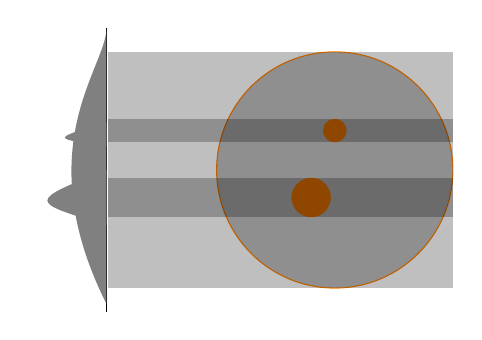
\begin{tikzpicture}[domain=3:3]  
		
		\fill[lightgray] (0.9,0.7) circle (1.5cm);
		
		\draw [rotate=90, yshift=2cm, - ](-1.1,0) -- (2.5,0); % s-Achse
		
		\fill[gray] [rotate=90, yshift=2cm] (-1,0) .. controls (1,1) and (2,0) .. (2.5,0);
		\fill[gray] [rotate=90, yshift=2cm] (0,0) .. controls (0.3,1)  .. (0.7,0);
		\fill[gray] [rotate=90, yshift=2cm] (1,0) .. controls (1.1,0.7)  .. (1.3,0);
		
		\draw[orange] (0.9,0.7) circle (1.5cm);
		\fill[orange] (0.9,  1.2) circle (.15cm);
		\fill[orange] (0.6, 0.35) circle (.25cm);
		
		\fill[nearly transparent] (-1.98,-0.8) rectangle (2.4,2.2);
		
		\fill[nearly transparent] (-1.98,0.1) rectangle (2.4,0.6);
		\fill[nearly transparent] (-1.98,1.05) rectangle (2.4,1.35);
		\begin{scope}[xshift=1cm]
		\end{scope}
		
		\end{tikzpicture} &	
		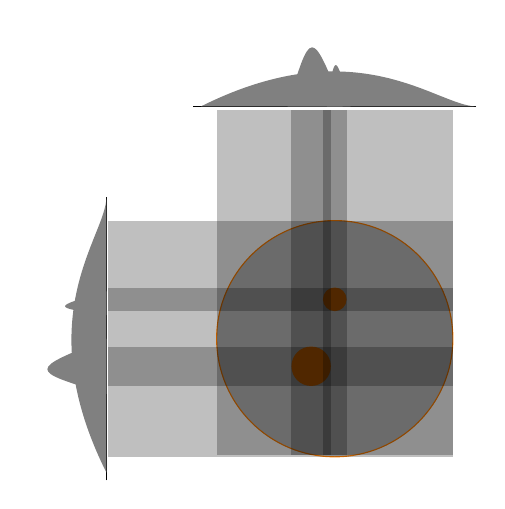
\begin{tikzpicture}[domain=3:3]  
		
		\fill[lightgray] (0.9,0.7) circle (1.5cm);
		
		\draw [rotate=90, yshift=2cm](-1.1,0) -- (2.5,0); % s-Achse
		
		\fill[gray] [rotate=90, yshift=2cm] (-1,0) .. controls (1,1) and (2,0) .. (2.5,0);
		\fill[gray] [rotate=90, yshift=2cm] (0,0) .. controls (0.3,1)  .. (0.7,0);
		\fill[gray] [rotate=90, yshift=2cm] (1,0) .. controls (1.1,0.7)  .. (1.3,0);
		
		\draw[orange] (0.9,0.7) circle (1.5cm);
		\fill[orange] (0.9,  1.2) circle (.15cm);
		\fill[orange] (0.6, 0.35) circle (.25cm);
		
		\fill[nearly transparent] (-1.98,-0.8) rectangle (2.4,2.2);
		
		\fill[nearly transparent] (-1.98,0.1) rectangle (2.4,0.6);
		\fill[nearly transparent] (-1.98,1.05) rectangle (2.4,1.35);
		\begin{scope}[xshift=1cm]
		\end{scope}
		
		\draw [rotate=0, yshift=3.65cm, xshift=0.2cm](-1.1,0) -- (2.5,0); % s-Achse
		
		\fill[gray] [rotate=0, yshift=3.65cm, xshift=0.2cm] (-1,0) .. controls (1,1) and (2,0) .. (2.5,0);
		\fill[gray] [rotate=0, yshift=3.65cm, xshift=0.3cm] (0,0) .. controls (0.3,1)  .. (0.7,0);
		\fill[gray] [rotate=0, yshift=3.65cm, xshift=-0.2cm] (1,0) .. controls (1.1,0.7)  .. (1.3,0);
		
		\fill[ nearly transparent] [rotate=90, xshift=1.1cm, yshift=-1.6cm] (-1.88,-0.8) rectangle (2.5,2.2);
		
		\fill[nearly transparent] [rotate=90, xshift=1.1cm, yshift=-0.95cm] (-1.88,0.1) rectangle (2.5,0.6);
		\fill[nearly transparent] [rotate=90, xshift=1.1cm, yshift=-2.1cm] (-1.88,1.05) rectangle (2.5,1.35);
		
		\end{tikzpicture}\\	
		(a) & (b) 
	\end{tabular}
	\caption{Das Prinzip der Bildrekonstruktion aus CT-Daten mit einer Rückprojektion~(a) und zwei Rückprojektionen~(b).} 
	\label{fig:1.2}
\end{figure}
%----------------------------------------------------------------------------------------
%	Ende der Grafik
%----------------------------------------------------------------------------------------

Ein Pionier der Tomographie, A. M. Cormack\footnote{\label{foot:1} Allan M. Cormack (1924-1998) südafrikanischer Physiker.}, veröffentlichte 1964 eine Arbeit über die mathematische Bestimmung der Dichten eines Objekts. Aus den Projektionsdaten konnte er die innere Dichteverteilung des Objekts bestimmen.

Der erste Prototyp eines CT-Scanners wurde vom G. N. Hounsfield\footnote{\label{foot:2} Godfrey N. Hounsfield (1919 - 2004) englischer Ingenieur.} im Jahr 1968 entwickelt. Seine Arbeit beruhte auf den Erkenntnissen von M. Cormack. Die Idee, der um das Objekt rotierenden Scanneinheit (Abb. \ref{fig:1.3}) findet man hier wieder. Vorerst konnten nur anatomische Präparate vermessen werden. Aber schon im Jahre 1972 entstehen erste klinische Untersuchungen mit einem Schädelscanner durch Hounsfield und Ambrose. 1973 werden Berichte über die Weichteildiagnostik des Gehirns mithilfe eines CT-Scanners veröffentlicht. Hinsichtlich der Nützlichkeit des CT-Verfahrens in der Medizin, wurden A. M. Cormack und G. N. Hounsfield im Jahre 1979 mit dem Nobelpreis für Medizin ausgezeichnet. 

In darauf folgenden Jahren entstand eine ganze Reihe von Generationen des CT-Scanners. Die Hauptunterschiede bestehen in der Komposition der Scanneinheit und dessen Technik, siehe auch \cite[Kap.\ 3]{Buzug04}. Heutzutage hat sich die dritte Genration am meisten durchgesetzt. Der prinzipielle Grundaufbau (Abb. \ref{fig:1.3}) dieses Scanners besteht darin, dass die Röntgenröhre und Detektor fest auf einem Ringkörper, einander gegenüber installiert sind. In der Mitte des Rings ist ein fest installierter Probetisch, sodass die Scanneinheit um diesen rotieren kann. Mittels dieser Konstruktion ist es möglich \textit{tomographische} Bilddaten aus allen Positionen um die Längsachse des Objekts aufzunehmen.
%----------------------------------------------------------------------------------------
%	Beginn der Grafik
%----------------------------------------------------------------------------------------
\begin{figure}[!h]
	
	\centering
	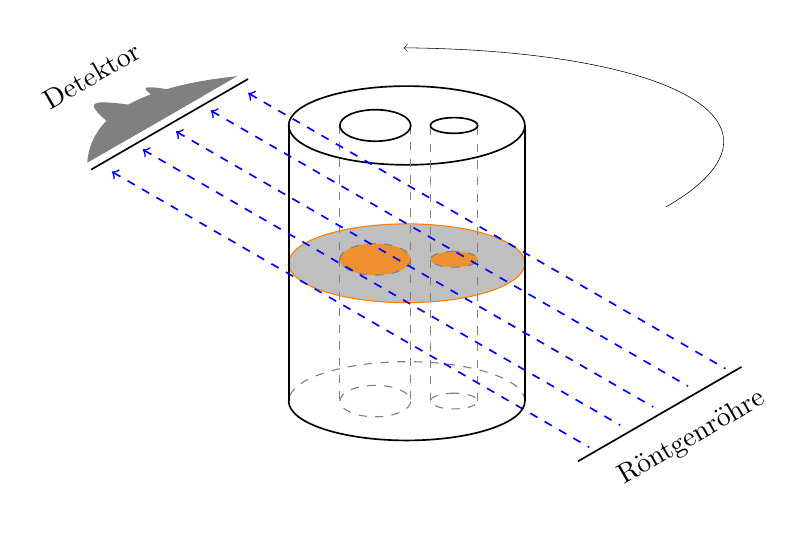
\begin{tikzpicture}
	%\draw[dashed,color=gray] [rotate=90, xshift=0cm, yshift=1.5cm] (-1,0) -- (4.4,0);% right line
	
	\draw[dashed,color=gray][rotate=90] (0,0) arc (-90:90:0.5 and 1.5);% top half of the bottom ellipse
	
	\draw[semithick][rotate=90] (4,1.5) arc (0:360:0.5 and 1.5);
	\draw[very thin, ->][rotate=95] (2.3,-2) arc (240:340:1.6 and 6);
	
	\fill[nearly transparent][rotate=90] (2.25,1.5) arc (0:360:0.5 and 1.5); % middle ellipse
	
	% inner lines
	\draw[dashed,color=gray] [rotate=90] (0,1.2) -- (3.5,1.2);% left line of inner small ellipse 
	\draw[dashed,color=gray] [rotate=90] (0,0.6) -- (3.5,0.6);% right line of the inner small ellipse
	
	\draw[dashed,color=gray] [rotate=90] (3.5, 2.35) -- (0, 2.35);% right line of the inner big ellipse
	\draw[dashed,color=gray] [rotate=90] (3.5, 1.45) -- (0, 1.45);% left line of the inner big ellipse
	
	% inner top ellipses
	\draw[semithick] [rotate=90] (3.5, .9) ellipse (0.1 and .3); % top small inner ellipse
	\draw[semithick] [rotate=90] (3.5, 1.9) ellipse (0.2 and .45); % top big inner ellipse
	
	% inner middle ellipses
	\fill[nearly opaque,color=orange] [rotate=90] (1.8, .9) ellipse (0.1 and .3);% middle small inner ellipse
	\fill[nearly opaque,color=orange] [rotate=90] (1.8, 1.9) ellipse (0.2 and .45); % middel big inner ellipse
	\draw[dashed,color=gray] [rotate=90] (1.8, .9) ellipse (0.1 and .3);% middle small inner ellipse
	\draw[dashed,color=gray] [rotate=90] (1.8, 1.9) ellipse (0.2 and .45); % middel big inner ellipse
	
	
	% inner bottom ellipses
	\draw[dashed,color=gray] [rotate=90] (0, .9) ellipse (0.1 and .3); % bottom small inner ellipse
	\draw[dashed,color=gray] [rotate=90] (0, 1.9) ellipse (0.2 and .45); % bottom big innerellipse
	
	\draw[color=orange][rotate=90] (2.25,1.5) arc (0:360:0.5 and 1.5); % middle ellipse
	
	%sids lines
	\draw[semithick] [rotate=90] (0,0) -- (3.5,0);% right line
	\draw[semithick] [rotate=90] (0,3) -- (3.5,3);% left line
	
	% Röntgenröhre
	\draw [semithick] [rotate=30, xshift=0.cm, yshift=-1.0cm](0.2,0) -- (2.6,0); % Röntgenröhre
	\draw  (1.5,-1.4) node [rotate=30, xshift=1.cm, yshift=0.5cm] { Röntgenröhre};
	
	\draw [semithick] [rotate=30, xshift=-3.5cm, yshift=5.3cm](0.2,0) -- (2.5,0); % Detektorachse
	\draw  (1.5,-1.4) node [rotate=30, xshift=-3.3cm, yshift=8.3cm] {Detektor};
	
	\draw [dashed, semithick, <-, blue] [rotate=150, , xshift=1.cm, yshift=0.1cm](5,0) -- (-2,0);
	\draw [dashed, semithick, <-, blue] [rotate=150, , xshift=0.8cm, yshift=-0.34cm](5,0) -- (-2,0);
	\draw [dashed, semithick, <-, blue] [rotate=150, , xshift=0.55cm, yshift=-0.75cm](5,0) -- (-2,0);
	\draw [dashed, semithick, <-, blue] [rotate=150, , xshift=0.3cm, yshift=-1.2cm](5,0) -- (-2,0);
	\draw [dashed, semithick, <-, blue] [rotate=150, , xshift=3.cm, yshift=-1.63cm](2,0) -- (-5,0);
	
	\fill[gray] [rotate=30, yshift=5.4cm, xshift=-3cm] (-0.3,0) .. controls (0.1,0.6) and (1,0.4) .. (1.9,0);
	\fill[gray] [rotate=30, yshift=5.4cm, xshift=-3cm] (0.3,0) .. controls (0,0.8)  .. (1,0);
	\fill[gray] [rotate=30, yshift=5.4cm, xshift=-3cm] (1,0) .. controls (0.7,0.6)  .. (1.4,0);
	
	\draw[semithick] [rotate=90] (0,0) arc (270:90:0.5 and 1.5);% bottom half of the bottom ellipse
	
	\end{tikzpicture}
	\caption{Prinzipieller Aufbau eines CT-Scanners der dritten Generation.}
	\label{fig:1.3}
\end{figure}
%----------------------------------------------------------------------------------------
%	Ende der Grafik
%----------------------------------------------------------------------------------------
Die oben beschriebene Rückprojektion aller tomographischen Daten (Projektionen) erzeugt ein Schnittbild. Erzeugt man mehrere Schnittbilder entlang der Längsachse des Objekts, so kann man diese der Reihe nach aufstellen und mithilfe programmiertechnischer Werkzeuge ein dreidimensionales Bild dieses Objekts gewinnen (Abb. \ref{fig:1.4}) .
%----------------------------------------------------------------------------------------
%	Beginn der Grafik
%----------------------------------------------------------------------------------------
\begin{figure}[h]
	\centering
	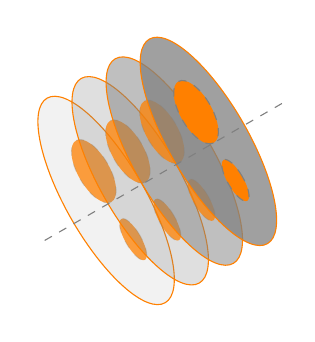
\begin{tikzpicture}
	
	\fill[very nearly transparent, color=gray][rotate=30] (2.25,1.5) arc (0:360:0.5 and 1.5); % middle ellipse
	
	% inner middle ellipses
	\fill[nearly opaque,color=orange] [rotate=30] (1.8, .9) ellipse (0.1 and .3);% middle small inner ellipse
	\fill[nearly opaque,color=orange] [rotate=30] (1.8, 1.9) ellipse (0.2 and .45); % middel big inner ellipse
	\draw[nearly transparent, dashed,color=gray] [rotate=30] (1.8, .9) ellipse (0.1 and .3);% middle small inner ellipse
	\draw[nearly transparent, dashed,color=gray] [rotate=30] (1.8, 1.9) ellipse (0.2 and .45); % middel big inner ellipse
	
	\draw[color=orange][rotate=30] (2.25,1.5) arc (0:360:0.5 and 1.5); % middle ellipse
	
	%--------- second slice
	
	\fill[nearly transparent, color=gray][rotate=30, xshift=0.5cm] (2.25,1.5) arc (0:360:0.5 and 1.5); % middle ellipse
	
	% inner middle ellipses
	\fill[nearly opaque,color=orange] [rotate=30, xshift=0.5cm] (1.8, .9) ellipse (0.1 and .3);% middle small inner ellipse
	\fill[nearly opaque,color=orange] [rotate=30, xshift=0.5cm] (1.8, 1.9) ellipse (0.2 and .45); % middel big inner ellipse
	\draw[nearly transparent, dashed,color=gray] [rotate=30, xshift=0.5cm] (1.8, .9) ellipse (0.1 and .3);% middle small inner ellipse
	\draw[nearly transparent, dashed,color=gray] [rotate=30, xshift=0.5cm] (1.8, 1.9) ellipse (0.2 and .45); % middel big inner ellipse
	
	\draw[color=orange][rotate=30, xshift=0.5cm] (2.25,1.5) arc (0:360:0.5 and 1.5); % middle ellipse
	
	%--------- third slice
	
	\fill[semitransparent, color=gray][rotate=30, xshift=1cm] (2.25,1.5) arc (0:360:0.5 and 1.5); % middle ellipse
	
	% inner middle ellipses
	\fill[nearly opaque, color=orange] [rotate=30, xshift=1cm] (1.8, .9) ellipse (0.1 and .3);% middle small inner ellipse
	\fill[nearly opaque, color=orange] [rotate=30, xshift=1cm] (1.8, 1.9) ellipse (0.2 and .45); % middel big inner ellipse
	\draw[nearly transparent, dashed,color=gray] [rotate=30, xshift=1cm] (1.8, .9) ellipse (0.1 and .3);% middle small inner ellipse
	\draw[nearly transparent, dashed,color=gray] [rotate=30, xshift=1cm] (1.8, 1.9) ellipse (0.2 and .45); % middel big inner ellipse
	
	\draw[color=orange][rotate=30, xshift=1cm] (2.25,1.5) arc (0:360:0.5 and 1.5); % middle ellipse
	
	%--------- fourd slice	
	
	\fill[nearly opaque, color=gray] [rotate=30, xshift=1.5cm] (2.25,1.5) arc (0:360:0.5 and 1.5); % middle ellipse
	
	% inner middle ellipses
	\fill[color=orange] [rotate=30, xshift=1.5cm] (1.8, .9) ellipse (0.1 and .3);% middle small inner ellipse
	\fill[color=orange] [rotate=30, xshift=1.5cm] (1.8, 1.9) ellipse (0.2 and .45); % middel big inner ellipse
	\draw[dashed,color=gray] [rotate=30, xshift=1.5cm] (1.8, .9) ellipse (0.1 and .3);% middle small inner ellipse
	\draw[dashed,color=gray] [rotate=30, xshift=1.5cm] (1.8, 1.9) ellipse (0.2 and .45); % middel big inner ellipse
	
	\draw[color=orange] [rotate=30, xshift=1.5cm] (2.25,1.5) arc (0:360:0.5 and 1.5); % middle ellipse
	
	\draw[dashed,color=gray] [rotate=30, xshift=0.8cm] (3.5, 1.45) -- (0, 1.45); % axisis
	
	\end{tikzpicture}
	\caption{Das Schichtmodell eines Objekts als Grundlage zur dreidimensionalen Rekonstruktion.}
	\label{fig:1.4}
\end{figure} 
%----------------------------------------------------------------------------------------
%	Ende der Grafik
%----------------------------------------------------------------------------------------

Im Folgenden gehen wir mehr auf die mathematisch-physikalischen Gegebenheiten der oben beschriebenen Situation ein. 

\section{Die Radon Transformation}
\label{cha:1.2}

Das Verständnis des mathematischen Problems der Bildrekonstruktion in der Computertomographie verlangt zunächst das Verständnis der Entstehung der tomographischen Bilddaten. Die Entstehung solcher Daten kann mithilfe eines mathematischen Modells nachvollzogen werden. Bekanntlich baut man das mathematische Modell auf physikalischen Annahmen auf. Die Abbildung \ref{fig:1.5} soll in diesem Fall als physikalisches Ausgangsmodell dienen. Wir nehmen an, dass der graue Kreis eine homogene Dichteverteilung besitzt. Unter weiteren Annahme sollen die Röntgenstrahlen sich geradlinig ohne Streuung in Richtung des Detektors ausbreiten.

Sei nun $f(x,y)$ die gesuchte Dichtefunktion, die auf einem Einheitskreis $\Omega = \{ (x,y) \in \R^2 \ | \ x^2 + y^2 \leq 1 \}$ definiert ist. Dass $f$ auf einem Kreis liegen soll, folgern wir aus der physikalischen Situation. Das Objekt wird aus einem bestimmten Radius um den Mittelpunkt der Scanneinheit gescannt, daher möchten wir, dass ein Objekt in die CT-Scanneinheit passt, gegebenenfalls muss die Scanneinheit skaliert werden.

Die blau gestrichelte Linie in Abbildung \ref{fig:1.5} stelle einen Röntgenstrahl dar. Wir möchten das Verhalten der Intensität entlang der Strahllinie an den Punkten $L_0$ und $L_0 + \Delta L$ beobachten. Wie schon erwähnt wurde, nimmt die Intensität $I$ der Röntgenstrahlen mit der Eindringtiefe in das Objekt ab. Das Verhalten ist in der Physik unter dem Namen \textit{Lambert-Beer’sches Gesetz} bekannt und besagt:
\begin{center}
	\textit{Die Intensitätsabnahme der Strahlung ist proportional zur Intensität. Der Proportionalitätsfaktor hängt von der Art der durchdrungenen Materie ab.}
\end{center}
\begin{equation}
	I(L_0 + \Delta L) - I(L_0) = - \alpha I(L_0).
	\label{equa:1.1}
\end{equation}
Der Proportionalitätsfaktor $\alpha$ ist durch das Produkt der Dichteverteilung entlang des Strahls, also $f(L)$ und seiner zurückgelegten Strecke $\parallel \Delta L\parallel$ gegeben. Hier wird angenommen, dass $f(L)$ die Eigenschaften des Materials in sich trägt. Insgesamt ergibt sich
\begin{equation}
	I(L_0 + \Delta L) - I(L_0) = -f(L) \parallel \Delta L \parallel I(L_0).
	\label{equa:1.2}
\end{equation}
Nimmt man an, dass die Gleichung (\ref{equa:1.2}) asymptotisch im Sinne $\parallel \Delta L \parallel \rightarrow 0$ verstanden werden kann, so kann die linke Seite von (\ref{equa:1.2}) als Ableitung von $I$ nach $L$ interpretiert werden und man schreibt:
\begin{equation}
	\lim_{\Delta L\rightarrow 0}\frac{I(L_0 + \Delta L) - I(L_0)}{\parallel \Delta L \parallel} = \frac{\partial I}{\partial L} = -f(L)I(L_0).
	\label{equa:1.3}
\end{equation}
Mit \ref{equa:1.3} liegt eine lineare Differentialgleichung (DGL) erster Ordnung vor. Diese DGL kann mithilfe einfacher analytischer Werkzeuge, wie Variablenseparation gelöst werden. 
%----------------------------------------------------------------------------------------
%	Beginn der Grafik
%----------------------------------------------------------------------------------------
\begin{figure}[!h]
	\centering
	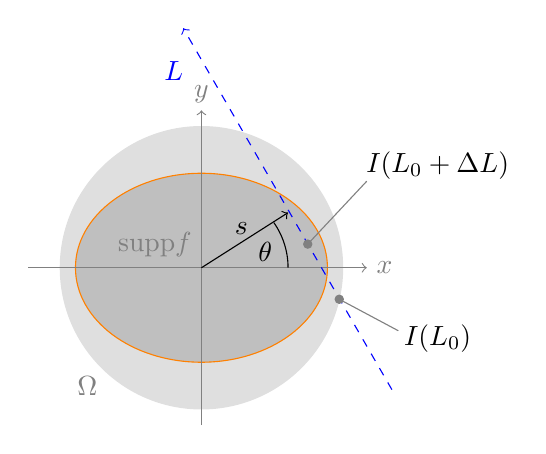
\begin{tikzpicture}

	\fill[nearly transparent, color=gray] (0.9,0) circle (1.8cm);
	
	\fill[lightgray] (0.9,0) ellipse (1.6cm and 1.2cm);	
	
	\draw[orange] (0.9,0) ellipse (1.6cm and 1.2cm);
	
	\draw [gray] [->](-1.3,0) -- (3,0); % x-Achse
	\draw [gray] (3, 0) node [right] {$x$};
	
	\draw [gray] [->](0.9,-2) -- (0.9,2); % y-Achse
	\draw [gray] (0.9, 2.2) node {$y$};
	
	\draw[gray](0.9, 0.3) node [left] {$\mbox{supp}f$};
	
	\draw[->] (0.9,0) -- (2, 0.7);
	\draw(1.2, 0.5)  node [right] {$s$};
	
	\draw [rotate=30, xshift=2.1cm, dashed, ->] [blue] (0,-3) -- (0,2.3); % strahl
	\draw [blue] (0.55, 2.5)  node {$L$};
	
	\draw(2,0) arc [start angle=0, end angle=35, radius=1cm];
	\draw(1.5, 0.2) node [right] {$\theta$};
	
	\draw [gray] (-0.8, -1.5) node [right] {$\Omega$};
	
	\draw(3.9, 1.3) node {$I(L_0 + \Delta L)$};
	\fill[gray](2.25, 0.3) circle [radius=0.06];
	\draw[-,thin,gray](2.25, 0.3) -- (3, 1.1);
	
	\draw(3.9, -0.9) node {$I(L_0)$};
	\fill[gray](2.65, -0.4) circle [radius=0.06];
	\draw[-,thin,gray](2.65, -0.4) -- (3.4, -0.8);
	
	\end{tikzpicture}	
	\caption{Intensitätsänderung der Röntgenstrahlung beim Passieren eines homogenen Objekts.}
	\label{fig:1.5}
\end{figure}
%----------------------------------------------------------------------------------------
%	Ende der Grafik
%----------------------------------------------------------------------------------------
Nach der Separation der Variablen in (\ref{equa:1.3}) und anschließender Integration bekommt man nun folgenden Ausdruck
\begin{equation}
	\ln(\frac{I_1}{I_0}) = -\int_{L_0}^{L_1} f(L) \mbox{d} L.
	\label{equa:1.4}
\end{equation}
Durch das Exponentieren von (\ref{equa:1.4}) gelangt man zu dem \textit{Lambert-Beer’schen Gesetz} $I(L_1) = I_0 e^{-\int_{L_0}^{L_1} f(L) \mbox{d} L}$. Jedoch für die Zwecke der Computertomographie interessiert man sich für etwas von (\ref{equa:1.4}) abgewandelte Darstellung
\begin{equation}
	\ln(\frac{I_0}{I_1}) = \int_{L_0}^{L_1} f(L) \mbox{d} L.
	\label{equa:1.5}
\end{equation} 
Die rechte Seite in (\ref{equa:1.5}) liefert einen Summenwert von $f$ entlang der Geraden $L$ (Abb. \ref{fig:1.6}), die wie folgt parametrisiert werden kann:
\begin{equation}
	\begin{matrix}
		L(s, \theta, t) & = & s\begin{pmatrix} \cos(\theta) \\ \sin(\theta) \end{pmatrix} & + & t\begin{pmatrix} -\sin(\theta) \\ \cos(\theta)  \end{pmatrix} \\ \\
		& = & s\omega(\theta) & + & t\omega^{\perp}(\theta)
	\end{matrix} \ , \ \ s, t \in \R; \ \theta \in [0,\pi].
	\label{equa:1.6}
\end{equation}
Betrachtet man alle Geraden, die den Einheitskreis schneiden, dann ergibt sich folgende Menge
\begin{equation}
	G = \{ L(s, \theta, t) \ | \ |s| \leq 1, \  \theta \in [0,\pi] \ t \in [-\gamma(s), \gamma(s)] \}.
	\label{equa:1.7}
\end{equation}
Wobei $\gamma(s)$ den Parameter $t$ für (\ref{equa:1.6}) festlegt und folgendermaßen definiert werden kann
\begin{equation}
	\gamma(s) = \left\{ \begin{matrix}
	\sqrt{1 - s^2} & : & |s| \leq 1 \\ 
	0 & : & \mbox{sonst}
	\end{matrix}.
	\right.
	\label{equa:1.8}
\end{equation}
Die Gleichung (\ref{equa:1.8}) liefert nun die Integrationsgrenzen für (\ref{equa:1.5}). Da die Werte von $\pm\gamma(s)$ genau die Schnittpunkte von $L$ mit $\Omega$ liefern und  $\mbox{supp} f$\footnote{\label{foot:3} Mit $\mbox{supp} f$ (Support) ist der Träger einer Funktion $f$ gemeint. Def.: $\mbox{supp} f := \overline{ \{ x \in \Omega | f(x) \neq 0 \} } $} $\subseteq \Omega$, heißt es insgesamt, dass nur die Werte von $L \subset \mbox{supp} f$ bei der Integration von (\ref{equa:1.5}) berücksichtigt werden.

Kehren wir zur Gleichung (\ref{equa:1.5}) zurück und betrachten die Abbildung \ref{fig:1.6}, werden wir feststellen, dass die Funktion $f$ über den Parameter $t$ integriert werden muss. Hierzu bedarf es einer Variablentransformation:
\begin{equation}
	\begin{matrix}
		|(J(L))| = \left|\begin{pmatrix} \cos(\theta) & \sin(\theta)\\ -\sin(\theta) & \cos(\theta) \end{pmatrix}\right| = 1 \\ \\
		\mbox{und} \\ \\
		\mbox{d}L = \mbox{det}(J(L)) \mbox{d}t .
	\end{matrix}
	\label{equa:1.9}
\end{equation}
%----------------------------------------------------------------------------------------
%	Beginn der Grafik
%----------------------------------------------------------------------------------------
\begin{figure}[!h]
	\centering
	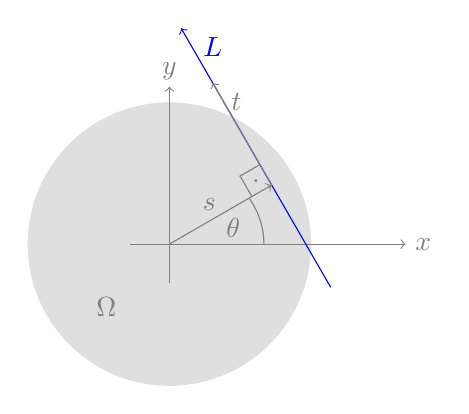
\begin{tikzpicture}
	
	\fill[nearly transparent, color=gray] (0,0) circle (1.8cm);
	
	\draw [gray] [->](-0.5,0) -- (3,0); % x-Achse
	\draw [gray] (3, 0) node [right] {$x$};
	
	\draw [gray] [->](0,-0.5) -- (0,2); % y-Achse
	\draw [gray] (0, 2.2) node {$y$};
	
	\draw [rotate=30, xshift=1.5cm, ->] [blue] (0,-1.5) -- (0,2.3); % strahl	
	\draw [blue] (0.55, 2.5)  node {$L$};%{$\omega^{\perp}$};
	
	\draw [rotate=30, xshift=1.5cm, ->] [gray ] (0,0) -- (0,1.5);
	\draw [gray] (0.85,1.8) node {$t$}; 
	
	\draw [xshift=1.05cm, yshift=0.6cm, rotate=120, - ] [gray] (0,0) -- (0.3,0);
	\draw [xshift=0.89cm, yshift=0.86cm, rotate=30, - ] [gray] (0,0) -- (0.3,0);
	\draw [gray] (1.1, 0.8)  node {$.$};
	
	\draw [rotate=30] [gray] [->] (0,0) -- (1.5, 0);
	\draw [gray] (0.3, 0.5)  node [right] {$s$};
	
	\draw [gray] (1.2,0) arc [start angle=0, end angle=35, radius=1cm];
	\draw [gray] (0.6, 0.2) node [right] {$\theta$};
	
	\draw [gray] (-0.8, -0.8) node {$\Omega$};
	
	\end{tikzpicture}
	\caption{Parametrisierung des Strahls $L$ auf dem Gebiet $\Omega$. }
	\label{fig:1.6}
\end{figure}
%----------------------------------------------------------------------------------------
%	Ende der Grafik
%----------------------------------------------------------------------------------------

Mit den obigen Abmachungen haben wir nun alles Nötige in der Hand, um die Radon\footnote{\label{foot:4} Johann Karl August Radon (1887-1956) österreichischer Mathematiker.} Transformation angeben zu können. 
\begin{Definition}
	Sei nun $f:\Omega \subseteq \R^2 \rightarrow \R$ eine integrierbare Funktion, dann ist ihre Radon Transformation durch
	\begin{equation}
		\mathcal{R}f(s,\theta) := \int\limits_{-\gamma(s)}^{\gamma(s)} f(s\omega(\theta) + t\omega^{\perp}(\theta)) \mbox{d}t
		\label{equa:1.10}
	\end{equation}
	definiert. Hier ist $\Omega = \{ (x,y) \in \R^2 \ | \ x^2 + y^2 \leq 1 \}$.
	\label{def.1}
\end{Definition}

\begin{Bemerkung}
	$\mathcal{R}$ wird als Integraloperator oder einfach als Operator bezeichnet.
	\label{bem:1} 
\end{Bemerkung}

Die Gleichung (\ref{equa:1.10}) trägt das Wesen der Computertomographie in sich und gehört in den Bereich der Integraltransformationen. In der Tat ist man aber an der Inversion von $\mathcal{R}$ interessiert. Das wird klarer, wenn man (\ref{equa:1.10}) etwas anders auffasst:
\begin{equation}
	p(s,\theta) = \mathcal{R}f(s,\theta).
	\label{equa:1.11}
\end{equation}
Somit stellt $p(s,\theta)$ in (\ref{equa:1.11}) genau die Projektion einer unbekannten Dichteverteilung entlang eines Röntgenstrahls $L(s,\theta)$ dar. Da die Projektionen als Messwerte beim CT-Verfahren entstehen, möchte man $f$ folgendermaßen wiedergewinnen 
\begin{equation}
	f(x) = \mathcal{R}^{-1}p(x).
	\label{equa:1.12}
\end{equation}
Jedoch offenbaren sich einige mathematische Hürden bei der Inversion von (\ref{equa:1.10}), was die Rekonstruktion von $f$ aus den Projektionsdaten schwierig macht. Um die dahinterstehende Problematik besser verstehen zu können, untersuchen wir zunächst die Eigenschaften von (\ref{equa:1.10}).

\subsection{Kleiner Einschub über $L^2$-Raum}
\label{cha:1.2.1}

Um den Operator $\mathcal{R}$ untersuchen zu können, sollte man wissen auf welchen Räumen er operiert. Dieses Wissen erlaubt uns Aussagen über die Stetigkeit, Kompaktheit und auch über die Singulärwertzerlegung (SWZ) von $\mathcal{R}$ zu treffen. Besonders wichtig ist die SWZ, denn anhand dieser ergibt sich eine Möglichkeit den Operator $\mathcal{R}$ zu invertieren. Zudem wollen wir im nächsten Kapitel die Schlechtgestelltheit des computertomographischen Problems diskutieren, welche die Eigenschaften der SWZ benutzt.

In Bezug auf das hier vorgestellte Rekonstruktionsproblem der Computertomographie betrachten wir Funktionen auf dem Gebiet $\Omega \subset \R^2$. Wir setzen voraus, dass die Funktionen auf $\Omega$ integrierbar sind. Wie dieser Sachverhalt zu verstehen ist, wollen wir kurz und grob andeuten.

Zunächst klären wir den Begriff der Integrierbarkeit einer Funktion im Sinne von Lebesgue\footnote{Henri Léon Lebesgue (1875-1941) französischer Mathematiker.}. Das Lebesgue-Integral wird für Funktionen auf einem geeigneten Maßraum definiert. Ein Maßraum ist durch ein Tripel $( \Omega, \mathcal{A}, \lambda)$ gegeben.

Eine sogenannte $\sigma$-\textit{Algebra} $\mathcal{A} \subset \mathcal{P}(\Omega)$ auf $\Omega$ ist ein Mengensystem bestehend aus Teilmengen von $\Omega$. $\mathcal{A}$ besitzt folgende Eigenschaften: (\lowroman{1}). Jede endliche oder abzählbar unendliche Vereinigung oder jeder Durchschnitt der Elemente aus $\mathcal{A}$ liegen wieder in $\mathcal{A}$, sowie $\Omega$ und $\emptyset$. (\lowroman{2}). Die Komplemente der Elemente aus $\mathcal{A}$, also $\forall A \in \mathcal{A} : \Omega \setminus A = A^\mathrm{C} \in \mathcal{A}$ , liegen auch in $\mathcal{A}$.

Nun suchen wir eine Funktion, die allen Elementen $A$ aus $\mathcal{A}$ eine positive Zahl zuordnet, also $\lambda(A) \in [0, \infty]$. Somit beschreibt $\lambda$ das Maß einer Menge in $\mathcal{A}$. Im Falle $\Omega \subset \R^2$ ordnet $\lambda$ den Flächeninhalt einer Teilmenge von $\Omega$ zu. Des Weiteren hat $\lambda$ folgende Eigenschaften: (\lowroman{1}): $\lambda(\emptyset) = 0$ und (\lowroman{2}): die $\sigma$-\textit{Additivität}, das heißt für paarweise disjunkte Mengen $(A_n)_{n \in \N}$ aus $\mathcal{A}$ gilt
 
\[ \lambda \left(  \bigcup\limits_{n=1}^{\infty} A_n \right) = \sum\limits_{n = 1}^{\infty} \lambda(A_n).\]  

Nun gilt per Definition \textit{messbarer Abbildungen} zwischen zwei Maßräumen, dass die Urbilder messbarer Mengen messbar sind. Das heißt $f:(X_1, \mathcal{A}_1) \rightarrow (X_2, \mathcal{A}_2)$ ist messbar, wenn für alle $A_{2_j} \in \mathcal{A}_2$ gilt $f^{-1}(A_{2_j}) \in \mathcal{A}_1$. 

Um den Begriff der Integrierbarkeit im Sinne von Lebesgue einführen zu können, fehlt uns noch der Begriff der Borel\footnote{Émile Borel (1871-1956)  französischer Mathematiker.}-$\sigma$-Algebra. Dazu benutzen wir für uns relevante mengen $\R$ und $\R^2$. Das ist insofern klar, weil die gesuchten Dichtefunktionen in einem Punkt $x \in \Omega \subset \R^2$ einen skalaren Wert $f(x) \in \R$ liefern. Noch legen wir fest, dass die Werte der Funktionen auf $\Omega$ immer positiv sind, also $f(x) \in \R^+$, denn es gibt keine negativen Dichten. Betrachten wir den topologischen Raum $(\R,\mathcal{T})$, hier stellt $\mathcal{T}$ \footnote{
Sei $X$ eine Menge, dann ist $\mathcal{T} \subset 2^{X}$ eine Topologie auf X, falls folgendes gilt:
\begin{itemize}
	\item[(i)] $\emptyset , X \subset \mathcal{T}$. 
	\item[(ii)] $ A,B \subset X \in \mathcal{T} \Rightarrow A \cap B \in \mathcal{T}$.
	\item[(iii)] $\{ A_{_i}\}_{_{i \in I}} \in \mathcal{T} \Rightarrow \bigcup\limits_{i \in I} A_{_i} \in \mathcal{T}$ 
\end{itemize}
So nennt man das Paar $(X, \mathcal{T})$ ein topologischer Raum. Alle Elemente von $\mathcal{T}$ sind offene Mengen.}
ein System von offenen Mengen von $\R$ dar, dann heißt $\mathcal{B}(\R)$ die von $\mathcal{T}$ erzeugte $\sigma$-Algebra auf $\R$, die Borel-$\sigma$-Algebra. $\mathcal{B}(\R)$ ist die kleinste Algebra, die $\mathcal{T}$ enthält. Das bringt uns ein Vorteil bezüglich der Messbarkeit, denn somit erhalten wir die größtmögliche Menge messbarer Mengen von $\R$. Für $\R^2$ gilt das Obere auch.

Im letzten Schritt definieren wir die sogenannten positiven Treppenfunktionen $h^+:(\Omega, \mathcal{B}(\Omega)) \rightarrow (\R, \mathcal{B}(\R))$, die endlich viele Werte $c_j \in \R_{0}^{+}, \ j \in [1,n], \ n \in \N$ auf $\Omega$ annehmen. Auf diese Weise ist es möglich das Integral über $h^+$ folgendermaßen anzugeben:

\[ \mathcal{I}(h^+) = \sum\limits_{j = 1}^{n} c_j \lambda({A_j}), \ \ \mbox{für } A_j \in \mathcal{B}(\Omega).\]

Jetzt können wir das Lebesgue-Integral einer messbaren Funktion $f: \Omega \rightarrow \R^+$ definieren, indem wir die Funktion $f$ `von unten' mit Treppenfunktionen approximieren:
\begin{Definition}
	Sei  $f: \Omega \rightarrow \R^+$ messbar, dann ist sie integrierbar im Sinne von Lebesgue, wenn gilt
	\[ \int\limits_{\Omega} f(x) = \sup\{ \mathcal{I}(h^+) | \forall x \in \Omega : h^+(x) \leq f(x) \} < \infty.\]
	\label{def.2}
\end{Definition}
\begin{Bemerkung}
	Im Falle einer Lebesgue-Integrierbarkeit spricht man meistens davon, dass eine Funktion Integrierbar ist. Streng genommen müsste man das Lebesgue-Integral für beliebige Funktionen $f:\Omega \rightarrow \R$ mit einer geeigneten Fortsetzung einführen, um dem Begriff der Integrierbarkeit gerecht zu werden. Aber die Definition \ref{def.2} reicht uns, um das Prinzip der Integration verstanden zu haben. 
	\label{bem:2}
\end{Bemerkung}
Nun sind wir im Stande den \textit{Raum der quadratintegrierbarer Funktionen} folgendermaßen zu definieren:
\begin{equation}
	\mathcal{L}^{2}(\Omega, \mathcal{A}, \lambda) = \{ f : \Omega \rightarrow \R \ | \ f \mbox{ ist integrierbar und } \int \limits_{\Omega} |f(x)|^2 \mbox{d}x \leq \infty \}.
	\label{equa:1.13}
\end{equation}
Versehen wir den Raum $\mathcal{L}^{2}(\Omega, \mathcal{A}, \lambda)$ mit einer Norm
\begin{equation}
	\Vert f \Vert_2 := \ < f, f >^{\frac{1}{2}} \ = \left( \int |f(x)|^2 \mbox{d}x \right)^{\frac{1}{2}}, \ \ x \in \Omega,
	\label{equa:1.14}
\end{equation}
so erhalten wir den Raum $L^2(\Omega, \mathcal{A}, \lambda)$ (einfach $L^2(\Omega)$), also den \textit{Hilbertraum der quadratintegrierbaren Funktionen}. 

Im Allgemeinen ist $L^2(\Omega)$ ein unendlichdimensionaler Vektorraum über dem Körper der komplexen Zahlen, der bezüglich der durch das Skalarprodukt induzierten Norm vollständig ist.

Kehren wir zurück, zu den gesuchten Funktionen auf einer Kreisscheibe $\Omega$, dann sei das Urbild des Operators $\mathcal{R}$ genau die Menge $L^2(\Omega)$. Das Bild von $\mathcal{R}$ liegt jedoch auf einem halben Zylinder $Z := [0, \pi] \times [-1,1]$. Der Grund hierfür ist ein technischer, denn bei Projektionen über den ganzen Durchmesser einer Kreisfläche auf einem Intervall von $0$ bis $2\pi$, entstehen redundante Daten, also reichen die Projektionen von $0$ bis $\pi$. 

Des Weiteren  wissen wir an dieser Stelle noch nicht wohin $\mathcal{R}$ den Raum $L^2(\Omega)$ abbildet. Aber wie oben schon erwähnt wurde, wollen wir später die SWZ von $\mathcal{R}$ angeben, dafür muss ein \textit{adjungierter} Operator $\mathcal{R^*}$ zu $\mathcal{R}$ existieren\footnote{\label{foot:5} Der Grund weshalb $\mathcal{R^*}$ existieren muss ist folgender: Es kann nicht vorausgesetzt werden, dass $\mathcal{R}$ selbstadjungiert ist, wonach der \textit{Spektralsatz für selbstadjungierte Operatoren} für $\mathcal{R}$ nicht gelten würde. Aber für $\mathcal{R}\mathcal{R^*}$ funktioniert der Satz schon, da $\mathcal{R}\mathcal{R^*} = (\mathcal{R}\mathcal{R^*})^* = \mathcal{R^*}\mathcal{R}$ gelte.}. Um das zu bewerkstelligen, muss man fordern, dass der Bildraum sowie der Kern von $\mathcal{R}$ Orthogonalbasen besitzen sollen, was auch einen Skalarprodukt impliziert. Hieraus kann eine Vermutung aufgestellt werden, dass $\mathcal{R}$ $L^2(\Omega)$ nach $L^2(Z)$ abbilden soll, weil eben $L^2$ Räume der Forderung gerecht sind. Somit erhalten wir insgesamt
\begin{equation}
	\mathcal{R} : L^2(\Omega) \rightarrow L^2(Z).
	\label{equa:1.15}
\end{equation}
Mit (\ref{equa:1.15}) kann man die Eigenschaften des Operators $\mathcal{R}$ gut untersuchen.

\subsection{Eigenschaften der Radon Transformation}
\label{cha:1.2.2}

In diesem Kapitel sollen einige Eigenschaften des Operators $\mathcal{R}$ erarbeitet werden. Anhand der Eigenschaften von $\mathcal{R}$ kann die Problematik der Gleichung (\ref{equa:1.12}) besser verstanden werden. Zunächst zeigen wir die Linearität von $\mathcal{R}$. 
\subsubsection{Linearität von $\mathcal{R}$}
$\mathcal{R}$ ist linear, denn für $f, g \in L^2(\Omega)$ beliebig,  ergibt sich 
\begin{equation}
	\begin{split}
		\mathcal{R}( \alpha f + \beta g) & \stackrel{\mbox{\scriptsize Def.}\ref{def.1}}{=}  \int\limits_{-\gamma(s)}^{\gamma(s)} \left( \alpha f + \beta g\right ) \mbox{d}t\\
		& \stackrel{\mbox{\scriptsize Lin.}}{=} \alpha \int\limits_{-\gamma(s)}^{\gamma(s)} f\mbox{d}t  +  \beta \int\limits_{-\gamma(s)}^{\gamma(s)} g \mbox{d}t\\
		& = \alpha \mathcal{R} f +  \beta \mathcal{R} g .
	\end{split}
	\label{equa:1.16}
\end{equation}
Der Übersichtlichkeit halber wurden in (\ref{equa:1.16}) die Argumente weggelassen, also für alle $f \in \Omega$ gilt $f = f(s\omega(\theta) + t\omega^{\perp}(\theta))$.

\subsubsection{Stetigkeit von $\mathcal{R}$}

Mit dem obigen Ergebnis kann man die Theorie der linearen Operatoren in normierten Räumen auf $\mathcal{R}$ anwenden. Nun wollen wir die Stetigkeit von $\mathcal{R}$ überprüfen.
\begin{lemma}
	Der Operator $R : L^2(\Omega) \rightarrow L^2(Z)$ ist stetig.
	\label{lemma:1}
\end{lemma}
\begin{proof}
	Das Ziel ist zu zeigen, dass das Bild von $\mathcal{R}$ beschränkt ist. Demnach ist jeder linearer beschränkter Operator stetig (s.a. \cite[S.82]{Burg91}). Wir führen den Beweis in zwei Schritten durch. Zuerst geben wir eine Abschätzung für $|\mathcal{R} f(s,\theta)|^2$ und dann für $\Vert \mathcal{R} \Vert_2$.
	\begin{enumerate}
		\item[\lowroman{1}.] Sei nun $f \in L^2(\Omega)$ beliebig, dann gilt mit Benutzung der Cauchy-Schwarzschen Ungleichung für Integrale
		\begin{equation}
			\begin{split}
				|\mathcal{R} f(s,\theta)|^2 & = \left| \ \int\limits_{-\gamma(s)}^{\gamma(s)} f(s\omega(\theta) + t\omega^{\perp}(\theta)) \mbox{d}t \ \right|^2 \\
				& \leq \int\limits_{-\gamma(s)}^{\gamma(s)} 1 \mbox{d}t \int\limits_{-\gamma(s)}^{\gamma(s)} |f(s\omega(\theta) + t\omega^{\perp}(\theta))|^2 \mbox{d}t\\
				& = 2 \gamma(s) \int\limits_{-\gamma(s)}^{\gamma(s)} |f(s\omega(\theta) + t\omega^{\perp}(\theta))|^2 \mbox{d}t.
			\end{split}
			\label{equa:1.17}
		\end{equation}
		Aus der Gleichung (\ref{equa:1.8}) wissen wir, dass $\gamma(s) \leq 1$ ist, damit können wir (\ref{equa:1.18}) weiter abschätzen
		\begin{equation}
			\begin{split}
				|\mathcal{R} f(s,\theta)|^2 & \leq \ 2 \gamma(s) \int\limits_{-\gamma(s)}^{\gamma(s)} |f(s\omega(\theta) + t\omega^{\perp}(\theta))|^2 \mbox{d}t \\
				& \stackrel{ ( \ref{equa:1.8} ) }{\leq} 2 \int\limits_{-\gamma(s)}^{\gamma(s)} |f(s\omega(\theta) + t\omega^{\perp}(\theta))|^2 \mbox{d}t.
			\end{split}
			\label{equa:1.18}
		\end{equation}
		\item[\lowroman{2}.] Mit (\ref{equa:1.18}) lässt sich das Skalarprodukt $\Vert \mathcal{R} f(s,\theta) \Vert_{L^2(Z)}^2$ abschätzen:
		\begin{equation}
			\begin{split}
				\Vert \mathcal{R} f(s,\theta) \Vert_{L^2(Z)}^2 & = \int\limits_{0}^{\pi} \int\limits_{-1}^{1} \ |\mathcal{R} f(s,\theta)|^2 \ \mbox{d}s \mbox{d}\theta \\
				& \stackrel{(\ref{equa:1.18})}{\leq} 2 \int\limits_{0}^{\pi} \int\limits_{-1}^{1} \left( \int\limits_{-\gamma(s)}^{\gamma(s)} |f(s\omega(\theta) + t\omega^{\perp}(\theta))|^2 \mbox{d}t \right) \mbox{d}s \ \mbox{d}\theta\\
				& = 2 \int\limits_{0}^{\pi} \left( \int\limits_{-1}^{1} \ \int\limits_{-\gamma(s)}^{\gamma(s)} |f(s\omega(\theta) + t\omega^{\perp}(\theta))|^2 \mbox{d}t \ \mbox{d}s \right) \mbox{d}\theta\\
				& = 2 \int\limits_{0}^{\pi} \left( \int\limits_{\Omega} \ |f(x)|^2 \mbox{d}x \right) \mbox{d}\theta\\
				& = 2\pi \Vert f \Vert_{L^2(\Omega)}^2.
			\end{split}
			\label{equa:1.19}
		\end{equation}
	\end{enumerate}	
	In der vorletzten Zeile von (\ref{equa:1.19}) wurde $s\omega(\theta) + t\omega^{\perp}(\theta) = x$ für ein festes $\theta$ gesetzt. Damit wurde der Integrationsbereich über $t$ und $s$ zu einem über $x$ gefasst, um insgesamt über ganz $\Omega$ integrieren zu können.  
	
	Nach dem Wurzelziehen aus (\ref{equa:1.19}), kommt man zur Erkenntnis, dass $\mathcal{R}$ beschränkt ist, nämlich $\Vert \mathcal{R} \Vert_2 \leq \sqrt{2\pi}$. Da $\mathcal{R}$ linear und beschränkt ist, dürfen wir auf seine Stetigkeit schließen.	
\end{proof}
Ist $\mathcal{R}$ linear und stetig so schreiben wir $\mathcal{R} \in  \mathscr{L}(L^2(\Omega), L^2(Z))$\footnote{\label{foot:6}$\mathscr{L}(X,Y)$ : Raum der stetigen linearen Abbildungen zwischen normierten Räumen $X$ und $Y$.}.

\subsubsection{Adjungierter Operator $\mathcal{R}$}

Da $\mathcal{R}$ stetig von $L^2(\Omega)$ nach $L^2(Z)$	abbildet, existiert zu $\mathcal{R}$ ein stetiger adjungierter Operator $\mathcal{R^*}$, d.h.
\begin{equation}
	\forall f \in L^2(\Omega) \wedge g \in L^2(Z) : \langle \mathcal{R}f, g \rangle_{L^2(\Z)} = \langle f, \mathcal{R^*}g \rangle_{L^2(\Omega)}.
	\label{equa:1.20}
\end{equation}
\begin{lemma}
	Der adjungierte Operator $\mathcal{R^*}$ zu $\mathcal{R}$ ist gegeben durch
	\begin{equation}
		\begin{split}
			& \mathcal{R^*} : L^2(Z) \rightarrow L^2(\Omega)\\
			& \mathcal{R^*} g(x) = \int\limits_{0}^{\pi} \ g(x^{T}\omega(\theta),\theta) \mbox{d}\theta.
		\end{split}
		\label{equa:1.21}
	\end{equation}
	\label{lemma:2}
\end{lemma}
\begin{Bemerkung}
	Bevor wir (\ref{equa:1.20}) für (\ref{equa:1.21}) zeigen, wollen wir die letztere Gleichung etwas besser in unsere Vorstellung einprägen. Sei dazu die Abb.\ref{fig:1.7} betrachtet. Wir wählen einen beliebigen Punkt $x = (\tilde{x}_1, \tilde{x}_2)^{T} \in \Omega$ und einen Wert $s \in [-1,1]$. So existiert folgende Beziehung zwischen $x$ und $s$
	\begin{equation}
		x^{T}\omega(\theta) = (s\cos(\theta), s\sin(\theta))\left( \begin{matrix} \cos(\theta) \\ \sin(\theta) \end{matrix}\right) = s(\cos^2(\theta) + \sin^2(\theta)) = s.
		\label{equa:1.22}
	\end{equation}
	Wobei wir gemäß der Abb.\ref{fig:1.7} für $x = (s\cos(\theta), s\sin(\theta))^T$ schreiben dürfen.
	
	(\ref{equa:1.21}) stellt eine Ungefilterte Rückprojektion dar. Man kann sich das folgendermaßen vorstellen. Für ein festes $x$ in der Ebene werden entsprechende Projektionen an der Stelle $s$ und Winkel $\theta$ zurück auf den Punkt $x$ projiziert. Nach der Addition der Projektionen auf $x$ über alle Winkel, bekommt man den Wert der ungefilterten Rückprojektion an dem Prunkt $x$.
	\label{bem:3}
\end{Bemerkung}
\begin{figure}[!h]
	\centering
	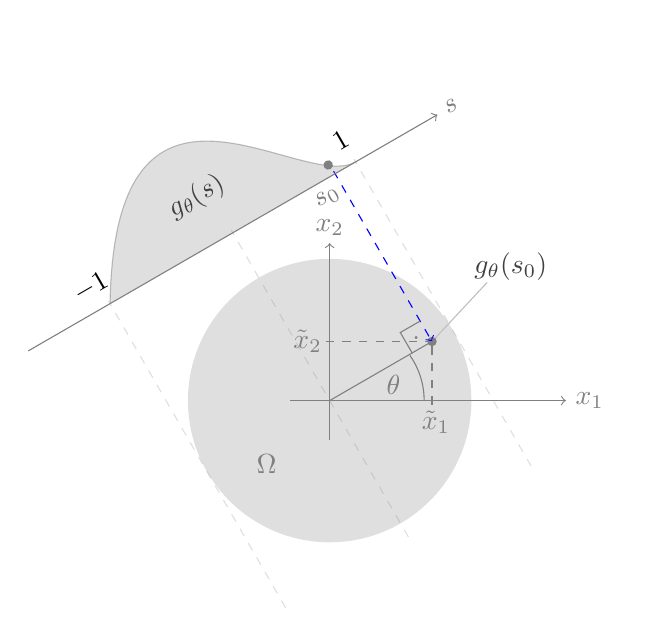
\begin{tikzpicture}	
	\fill[nearly transparent, color=gray] (0,0) circle (1.8cm);
	
	\draw [gray] [->](-0.5,0) -- (3,0); % x-Achse
	\draw [gray] (3, 0) node [right] {$x_1$};
	
	\draw [gray] [->](0,-0.5) -- (0,2); % y-Achse
	\draw [gray] (0, 2.2) node {$x_2$};
	
	\draw[lightgray](1.3,0.75) -- (2, 1.5);
	\fill[gray](1.3,0.75) circle [radius=0.06]; % ein Punkt		
	\draw [darkgray] (2.3, 1.7) node {$g_{\theta}(s_0)$};
	
	\draw [rotate=30, xshift=1.5cm, ->, dashed] [blue] (0,2.5) -- (0,0); % strahl
			
	
	\draw [xshift=1.05cm, yshift=0.6cm, rotate=120, - ] [gray] (0,0) -- (0.3,0);
	\draw [xshift=0.89cm, yshift=0.86cm, rotate=30, - ] [gray] (0,0) -- (0.3,0);
	\draw [gray] (1.1, 0.8)  node {$.$};
	
	\draw [rotate=30] [gray] [-] (0,0) -- (1.5, 0);
	
	\draw [dashed] [gray] (1.3,-0.05) -- (1.3,0.75); % x-Projektion
	\draw [gray] (1.35,-0.28)  node {$\tilde{x}_1$};
	
	\draw [dashed] [gray] (-0.05,0.75) -- (1.3,0.75); % y-Projektion		
	\draw [gray] (-0.28,0.75)  node {$\tilde{x}_2$};
	
	\draw [lightgray] [rotate=30, yshift=70] (-1.8,0) .. controls (0,3) and (1,0) .. (1.8,0);
	\fill [nearly transparent, color=gray] [rotate=30, yshift=70] (-1.8,0) .. controls (0,3) and (1,0) .. (1.8,0);

	\fill[ rotate=30, xshift=0.18cm, yshift=1.85cm, gray](1.3,0.75) circle [radius=0.06]; % ein Punkt
	
	\draw [rotate=30, xshift=0, yshift=70] [gray] [->] (-3,0) -- (3, 0);
	\draw [gray] (3.7, 0)  node [rotate=30, xshift=0, yshift=123] {$s$};
	
	\draw [gray] (0, 0)  node [rotate=30, xshift=1.55cm, yshift=2.25cm, left] {$s_0$};
	
	\draw [darkgray] (-0.2, 0)  node [rotate=30, yshift=85] {$g_{\theta}(s)$};		
	
	\draw [rotate=30, xshift=0cm, dashed] [nearly transparent, color=gray] (0,-2) -- (0,2.5); % punktiert Mitte
	\draw [rotate=30, xshift=1.8cm, dashed] [nearly transparent, color=gray] (0,-2) -- (0,2.5); % rechts punktiert
	\draw [rotate=30, xshift=-1.8cm, dashed] [nearly transparent, color=gray] (0,-2) -- (0,2.5); % links punktiert 
	
	\draw  (-1.8, 0) node [left, rotate=30, yshift=53]  {$-1$};
	\draw  (1.8, 0) node [right, rotate=30, yshift=105]  {$1$};
	
	\draw [gray] (1.2,0) arc [start angle=0, end angle=35, radius=1cm];
	\draw [gray] (0.6, 0.2) node [right] {$\theta$};
	
	\draw [gray] (-0.8, -0.8) node {$\Omega$};
	
	\end{tikzpicture}
	\caption{Ein Beispiel der Rückprojektion eines Projektionswerts $g_{\theta}(s_0)$ auf einen Punkt $x \in \Omega$. Mit $g_{\theta}(s)$ ist hier eine Projektion bei einem festen Winkel $\theta$ bezeichnet, also $g_{\theta}(s) = g(s,\theta)$.}
	\label{fig:1.7}
\end{figure}	  
\begin{proof}[Beweis von Lemma \ref{lemma:2}.]
Seien $f \in L^2(\Omega)$ und $g \in L^2(Z)$ beliebig, dann gilt
\begin{equation}
	\begin{split}
		\langle \mathcal{R} f, g \rangle_{L^2(Z)} & = \int\limits_{Z}^{} \left( \mathcal{R} f(s,\theta) \right) g(x^{T}\omega(\theta),\theta) \ \mbox{d}s \mbox{d}\theta \\
		& \stackrel{(\ref{equa:1.10})}{=} \int\limits_{0}^{\pi} \int\limits_{-1}^{1} \left( \int\limits_{-\gamma(s)}^{\gamma(s)}f(s\omega(\theta) + t\omega^{\perp}(\theta)) \mbox{d}t  \right) g(x^{T}\omega(\theta),\theta) \ \mbox{d}s \ \mbox{d}\theta.
		\end{split}
	\label{equa:1.23}
\end{equation}
An dieser Stelle machen wir eine Substitution in der rechten Seite von (\ref{equa:1.23}). Hier nutzen wir (\ref{equa:1.22}) aus und schreiben $x^T \omega(\theta) = \omega^T(\theta)x = s$. Dann bekommt man $g(x^{T}\omega(\theta),\theta) = g(\omega^T(\theta)x,\theta)$ und wir wollen die Funktion $f$ im Punkt $x$ betrachten, also $f(s\omega(\theta) + t\omega^{\perp}(\theta)) = f(x)$. Somit erhalten wir einen Integrationsbereich über $\Omega$. Nun führen wir (\ref{equa:1.24}) weiter:
\begin{equation}
	\begin{split}
		\langle \mathcal{R} f, g \rangle_{L^2(Z)} & = \int\limits_{0}^{\pi} \int\limits_{-1}^{1} \left( \int\limits_{-\gamma(s)}^{\gamma(s)}f(s\omega(\theta) + t\omega^{\perp}(\theta)) \mbox{d}t  \right) g(x^{T}\omega(\theta),\theta) \ \mbox{d}s \ \mbox{d}\theta \\
		& \stackrel{\mbox{\scriptsize Subst.}}{=}  \int\limits_{0}^{\pi} \left( \int\limits_{-1}^{1} \int\limits_{-\gamma(s)}^{\gamma(s)}f(x) g(\omega^T(\theta)x,\theta) \ \mbox{d}t \ \mbox{d}s \right) \mbox{d}\theta \\	
		& = \int\limits_{0}^{\pi} \int\limits_{\Omega} f(x) g(\omega^T(\theta)x,\theta) \ \mbox{d}x \ \mbox{d}\theta \\
		& = \int\limits_{\Omega} f(x) \left( \int\limits_{0}^{\pi} g(\omega^T(\theta)x,\theta) \ \mbox{d}\theta \right) \mbox{d}x  \\  
		& =\langle f, \mathcal{R^*} g \rangle_{L^2(\Omega)}.
	\end{split}
	\label{equa:1.24}
\end{equation}	 
Somit ist $\mathcal{R^*}$ adjungierter Operator der Radon Transformation und ist nach Satz von Schauder auch kompakt, wenn $\mathcal{R}$ kompakt ist. (\cite[S. 185]{Heuser75}).	 
\end{proof}

\subsubsection{Kompaktheit von $\mathcal{R}$}

Um die Kompaktheit von $\mathcal{R}$ zeigen zu können, werden wir an dieser Stelle einen Umweg einschlagen. Dafür ziehen wir ein Ergebnis aus \cite[S. 45]{Rieder03} heran. Es handelt sich um einen zu $\mathcal{R}$ adjungierten Operator $\tilde{\mathcal{R}}^*$ folgender Gestalt:
\begin{equation}
	\tilde{\mathcal{R}}^* : L^2(Z, \frac{1}{\gamma(s)}) \rightarrow L^2(\Omega).
	\label{equa:1.25}
\end{equation}
Hier wurde $\gamma(s)$ im Sinne der Gleichung (\ref{equa:1.8}) benutzt. Und der Raum $L^2(Z,\frac{1}{\gamma(s)})$ ist mit dem folgenden Skalarprodukt versehen
\begin{equation}
	\langle g,f \rangle = \int\limits_{Z} g \overline{f}\frac{1}{\gamma(s)}\mbox{d}s \mbox{d}\theta.
	\label{equa:1.26}
\end{equation}

Wir können festhalten dass der Operator $\mathcal{R'}:L^2(\Omega) \rightarrow  L^2(Z, \frac{1}{\gamma(s)})$ kompakt ist\footnote{Prinzipiell sind $\mathcal{R}$ und $\mathcal{R'}$ gleich, es ist derselbe Operator, der aber $L^2(\Omega)$ in einen anderen Raum abbildet. Die Bezeichnung $\mathcal{R}'$ führen wir ein, um uns Verwechslungen zu ersparen.}. Die Kompaktheit folgt eben aus der SWZ von $\mathcal{R}'$. Denn die Singulärwerte von $\mathcal{R}'$
\[
\sigma_j = 2\sqrt{\frac{\pi}{j + 1}}, \ \ j \in \N
\]
bilden eine Nullfolge, was nach einer längeren Rechnung aus \cite[S. 43]{Rieder03} folgt. Also schreiben wir $\mathcal{R}' \in \mathscr{K}(L^2(\Omega), L^2(Z,\frac{1}{\gamma(s)}))$\footnote{\label{foot:7}$\mathscr{K}(X,Y) = \{ A \in \mathscr{L}(X,Y) \ | \ A \mbox{ ist kompakt } \}$ }. 

Wir veranschaulichen die entstandene Situation in einem kommutativen Diagramm  
\begin{equation}
	\begin{xy}
	\xymatrix{
		L^2(\Omega) \ar[rr]^{\mathcal{R}} \ar@<2pt>[rd]^{\mathcal{R}'} &  & L^2(Z)\\
		&  L^2(Z, \frac{1}{\gamma(s)}) \ar@<2pt>[lu]^{\tilde{\mathcal{R}}^*} \ar[ru]_{\mbox{Id}}&
		}
	\end{xy}
	\label{equa:1.27}
\end{equation}
und stellen fest, dass $\mathcal{R}$ als eine Komposition zweier Abbildungen darstellbar ist. Hier bedeutet $\mbox{Id}$ die Identität auf $L^2(Z)$ dar. Der Unterschied zwischen $L^2(Z)$ und $L^2(Z,\frac{1}{\gamma(s)})$ besteht nur in der Definition des Skalarprodukts auf diesen beiden Räumen.

Insgesamt würde es heißen, dass wir die Komposition $\mbox{Id}\circ\mathcal{R}' = \mathcal{R}$ bezüglich der Kompaktheit beurteilen müssen. Dafür wird uns ein nützlicher Satz aus \cite[S. 27]{Rieder03} gute Dienste leisten (ohne Beweis) :
\begin{theorem}
	Seien $X, Y$ und $Z$ normierte Räume. Falls $A \in \mathscr{L}(X,Y)$ und $B \in \mathscr{K}(Y,Z)$ oder $A \in \mathscr{K}(X,Y)$ und $B \in \mathscr{L}(Y,Z)$, dann gilt $BA \in \mathscr{K}(X,Z)$.
	\label{satz:1}
\end{theorem}
Somit wollen wir zeigen, dass der Operator $\mbox{Id}:L^2(Z, \frac{1}{\gamma(s)}) \rightarrow L^2(Z)$ beschränkt ist, und somit auch stetig ist. Danach könnten wir den Satz \ref{satz:1} benutzen, um die Kompaktheit von $\mathcal{R}$ zu zeigen.

Sei nun $g(s,\theta) \in L^2(Z)$ beliebig, dann können wir folgende Abschätzung durchführen:
\begin{equation}
	\begin{split}
		\parallel \mbox{Id} \ g(s, \theta) \parallel_{L^2(Z)}^{2} & = \ \int \limits_{Z} |\mathcal{R}f(s, \theta)|^2 \mbox{d}s \mbox{d}\theta \\
		& \stackrel{(\ref{equa:1.26})}{\leq} \int \limits_{Z}  |\mathcal{R}f(s, \theta)|^2 \frac{1}{\gamma(s)} \ \mbox{d}s \ \mbox{d}\theta\\
		& = \ \parallel g(s, \theta) \parallel_{L^2(Z, \frac{1}{\gamma(s)})}^{2}.
	\end{split}
	\label{equa:1.28}
\end{equation}
Die letzte Abschätzung beruht auf der Kenntnis, dass  $\gamma(s) \leq 1$ für alle $s \in (-1,1)$, somit aber $\frac{1}{\gamma(s)} \geq 1$ gilt. Nun haben wir gezeigt, dass $\parallel \mbox{Id} \parallel_2 \leq 1$ beschränkt und demnach stetig ist. Also gilt $\mbox{Id} \in \mathscr{L}(L^2(Z, \frac{1}{\gamma(s)}), L^2(Z))$. Dieses Ergebnis ist für uns ausreichend um den Satz \ref{satz:1} benutzen zu können, d.h 
\begin{equation}
	\mathcal{R} \stackrel{(\ref{equa:1.27})}{=} \mbox{Id} \circ \mathcal{R}' \xLongrightarrow{\text{Satz \ref{satz:1}}} \mathcal{R} \in \mathscr{K}(L^2(\Omega), L^2(Z)).
	\label{equa:1.29}
\end{equation}

Nun sind wir am Ende dieses Kapitels angelangt und nach einigen Untersuchungen können wir festhalten, dass der lineare stetige Operator $\mathcal{R} : L^2(\Omega) \rightarrow L^2(Z)$ kompakt ist und einen kompakten adjungierten Operator $\mathcal{R^*}$ hat. Diese Ergebnisse spielen eine zentrale Rolle bei der Singulärwertzerlegung (SWZ) eines kompakten Operators und beleuchten das Problem der Invertierung solcher Operatoren sehr gut.

\subsubsection{Die Singulärwertzerlegung (SWZ) von $\mathcal{R}$}

Im Folgenden wird die allgemeine Form der SWZ des Operators $\mathcal{R}$ angegeben, eine konkrete wird in \cite[Kap. 2.5]{Rieder03} hergeleitet, jedoch aber nur für $\mathcal{R}'$. Um zu SWZ von $\mathcal{R}$ zu gelangen, ermittelt man zuerst die Eigenwerte und Eigenvektoren von $\mathcal{R}\mathcal{R^*} : L^2(Z) \rightarrow L^2(Z)$, die als Komposition kompakter Operatoren kompakt ist. Demnach gilt der \textit{Spektralsatz für selbstadjungierte kompakte Operatoren} \cite[S. 30]{Rieder03} und man bekommt 
\begin{equation}
	\mathcal{R}\mathcal{R^*}g = \sum\limits_{j=1}^{\infty} \lambda_j \langle g, v_j \rangle_{L^2(Z)} v_j, \ \ \mbox{für alle} \ \ g \in L^2(Z).
	\label{equa:1.30}
\end{equation}
Hier bildet $\{ \lambda_j \}_{j \in \N} \in \R$ eine Folge mit der absteigenden Anordnung der Eigenwerte $|\lambda_1| \geq |\lambda_2| \geq ... > 0$ und $\{ v_j\}_{j \in \N} \in L^2(Z)$ ein Orthonormalsystem in $\mbox{Kern}(\mathcal{R})^{\perp}$. Eine wichtige Tatsache ist, dass die Folge $\{\lambda_j\}_{j \in \N}$ entweder abbricht oder gegen Null konvergiert.

Die Singulärwerte und das Orthonormalsystem $\{u_j\}_{j \in \N}$ des Bildes von $\mathcal{R}$ bekommen wir aus
\begin{equation}
	\begin{split}
		(i). \ \sigma_j &:= \sqrt{\lambda_j}\\ 
		(ii). \ u_j	&:= \sigma_j^{-1}\mathcal{R}v_j
	\end{split}
	 , \ \  j \in \N.
	 \label{equa:1.31}
\end{equation}
Mit den Ergebnissen aus (\ref{equa:1.30}) und (\ref{equa:1.31}) kann nun die SWZ der Radon Transformation angegeben werden
\begin{equation}
	\mathcal{R}f = \sum\limits_{j = 1}^{\infty} \sigma_j \langle f, v_j\rangle_{L^2(\Omega)} u_j.
	\label{equa:1.32}
\end{equation}
Das Tripel $\{(\sigma_j, v_j, u_j)\}$ nennt man \textit{Singulärsystem} eines kompakten Operators und die Folgen $\{u_j\}_{j \in \N}$ und $\{ v_j\}_{j \in \N}$ bilden folgende Orthonormalsysteme
\begin{equation}
	\overline{\mbox{Span}\{u_j | j \in \N \} } = \overline{\mbox{Bild}(\mathcal{R})} \ \ \mbox{und} \ \ \overline{\mbox{Span}\{v_j | j \in \N \} } = \mbox{Kern}(\mathcal{R})^{\perp}.
	\label{equa:1.33}
\end{equation}

Die Gleichung (\ref{equa:1.32}) wird im nächsten Kapitel bei der Klärung des Begriffs \textit{schlecht gestellter Probleme} sehr hilfreich sein. 






